\documentclass[10pt, compress, aspectratio=169]{beamer}

\usetheme[numbering=fraction, progressbar=none, titleformat=smallcaps, sectionpage=none]{metropolis}

\usepackage{sourcecodepro}
\usepackage{booktabs}
\usepackage{array}
\usepackage{listings}
\usepackage{graphicx}
\usepackage[english]{babel}
\usepackage[scale=2]{ccicons}
\usepackage{url}
\usepackage{relsize}
\usepackage{wasysym}

\usepackage{pgfplots}
\usepgfplotslibrary{dateplot}

\definecolor{Base}{HTML}{191F26}
\definecolor{Accent}{HTML}{157FFF}

\setbeamercolor{alerted text}{fg=Accent}
\setbeamercolor{frametitle}{bg=Base}
\setbeamercolor{normal text}{bg=black!2,fg=Base}

\setsansfont[BoldFont={Source Sans Pro Semibold},
              Numbers={OldStyle}]{Source Sans Pro}

\lstset{ %
  backgroundcolor={},
  basicstyle=\ttfamily\footnotesize,
  breakatwhitespace=true,
  breaklines=true,
  captionpos=n,
  commentstyle=\color{Accent},
  escapeinside={\%*}{*)},
  extendedchars=true,
  frame=n,
  keywordstyle=\color{Accent},
  language=C++,
  rulecolor=\color{black},
  showspaces=false,
  showstringspaces=false,
  showtabs=false,
  stepnumber=2,
  stringstyle=\color{gray},
  tabsize=2,
  keywords={thrust,plus,device_vector, copy,transform,begin,end, copyin,
  copyout, acc, \_\_global\_\_, void, int, float, main, threadIdx, blockIdx,
  blockDim, if, else, malloc, NULL, cudaMalloc, cudaMemcpy, cudaSuccess,
  cudaGetLastError, cudaDeviceSynchronize, cudaFree, cudaMemcpyDeviceToHost,
  cudaMemcpyHostToDevice, const, data, independent, kernels, loop,
  fprintf, stderr, cudaGetErrorString, EXIT_FAILURE, for, dim3},
  otherkeywords={::, \#pragma, \#include, <<<,>>>, \&, \*, +, -, /, [, ], >, <}
}

\renewcommand*{\UrlFont}{\ttfamily\smaller\relax}

\graphicspath{{../../images/}}

\title{Parallel and Distributed Autotuning \\ for High-Performance Computing}
\author{\footnotesize Pedro Bruel \\ {\scriptsize \emph{phrb@ime.usp.br}}}
\institute{\includegraphics[height=2cm]{imelogo}\\[0.2cm] \emph{Institute of Mathematics and Statistics \\ University of São Paulo}}
\date{\scriptsize Qualifying Exam, October 30, 2017}

\begin{document}

\maketitle

\begin{frame}
    \frametitle{Outline}
    \setbeamertemplate{section in toc}[sections numbered]
    \tableofcontents[hideallsubsections]
\end{frame}

\section{Introduction}
\plain{Introduction}

\begin{frame}
    \frametitle{Autotuning: Configuring Hardware \& Software as a Search Problem}
    \begin{columns}[c]
        \column{.45\textwidth}
            \begin{block}{Hardware Configurations}
                \begin{itemize}
                    \item CPUs
                    \item GPUs
                    \item FPGAs
                    \item Supercomputers
                    \item $\dots$
                \end{itemize}
            \end{block}
            \begin{block}{Software Configurations}
                \begin{itemize}
                    \item Pthreads
                    \item OpenCL
                    \item MPI
                    \item Algorithms
                    \item $\dots$
                \end{itemize}
            \end{block}

        \column{.1\textwidth}
            \Huge{$\rightrightarrows$}

        \column{.45\textwidth}
            \begin{block}{}
                \begin{center}
                    \includegraphics[width=\columnwidth]{sample_search_space}
                    \alert{Search Problem}
                \end{center}
            \end{block}

    \end{columns}
\end{frame}

\begin{frame}
    \frametitle{Autotuning Systems: Multiple Approaches}
    \begin{table}
        \centering
        \begin{tabular}{@{}lll@{}}
            \toprule
            System & Domain & \alert{Technique} \\ \midrule
            ATLAS & Dense Linear Algebra & Exhaustive \\ \addlinespace
            INSIEME & Compiler & Genetic Algorithm \\
            TANGRAM & Heterogeneous Architectures & Breadth-First Search + Pruning \\
            Active Harmony & Runtime & Nelder-Mead \\
            ParamILS & \alert{Domain-Agnostic} & Stochastic Local Search \\
            CLTune & OpenCL kernels & Stochastic Local Search\\
            OPAL & \alert{Domain-Agnostic} & Direct Search \\ \addlinespace
            MILEPOST GCC & Compiler & Central DB + Machine Learning \\
            Apollo & GPU kernels & Decision Trees \\ \addlinespace
            \alert{OpenTuner} & \alert{Domain-Agnostic} & Ensemble \\
            Periscope & HPC Applications & Various \\
            \bottomrule
        \end{tabular}
    \end{table}
\end{frame}

\begin{frame}
    \frametitle{Autotuning Systems: Multiple Approaches}
    \begin{center}
        \includegraphics[width=.6\textwidth]{autotuning_strategies}
    \end{center}
\end{frame}

\begin{frame}
    \frametitle{Domain-Agnostic Autotuning}
    \begin{columns}[c]
        \column{.45\textwidth}
        \begin{block}{Problem Representation}
            \begin{itemize}
                \item Parameter \alert{types}
                \item \alert{User-definable cost function}
            \end{itemize}
        \end{block}

        \begin{block}{Robust Search Methods}
            \begin{itemize}
                \item \alert{Combinations} of techniques
                \item \alert{Model-Aided}
            \end{itemize}
        \end{block}

        \pause

        \column{.45\textwidth}
        \begin{block}{Limitations of Current Systems}
            \begin{itemize}
                \item Rely on \alert{multiple evaluations}
                \item \alert{Do not leverage parallelism}
            \end{itemize}
        \end{block}

    \end{columns}
\end{frame}

\begin{frame}
    \frametitle{Expected Contribution}
    \begin{columns}[c]
        \column{.45\textwidth}
        \begin{center}
            \includegraphics[width=\columnwidth]{logo}
        \end{center}

        \column{.45\textwidth}
        \begin{block}{NODAL}
            \begin{itemize}
                \item \alert{Domain-agnostic}
                \item \alert{Parallel \& distributed}
                \item \alert{Ensemble} of search techniques
                \item Guided by \alert{Design of Experiments}
            \end{itemize}
        \end{block}

    \end{columns}
\end{frame}

\begin{frame}
    \frametitle{Efforts for a Reproducible \& Open Research}
    \begin{columns}[t]
        \column{.45\textwidth}
            \begin{block}{Openness}
                \begin{itemize}
                    \item Publicly hosted software
                    \item Version control
                    \item Free software licenses
                    \item Copyright-free paper versions
                \end{itemize}
            \end{block}

        \column{.45\textwidth}
            \begin{block}{Reproducibility}
                \begin{itemize}
                    \item Publicly hosted data
                    \item Hardware \& Software specifications
                \end{itemize}
            \end{block}

    \end{columns}

    \pause

    \begin{center}
        Not all was open and reproducible, since we used proprietary software
        and hardware
    \end{center}
\end{frame}

\section{Algorithm Selection \& Autotuning}
\plain{Algorithm Selection \& Autotuning}

\begin{frame}
    \frametitle{The Algorithm Selection Framework}
    \begin{center}
        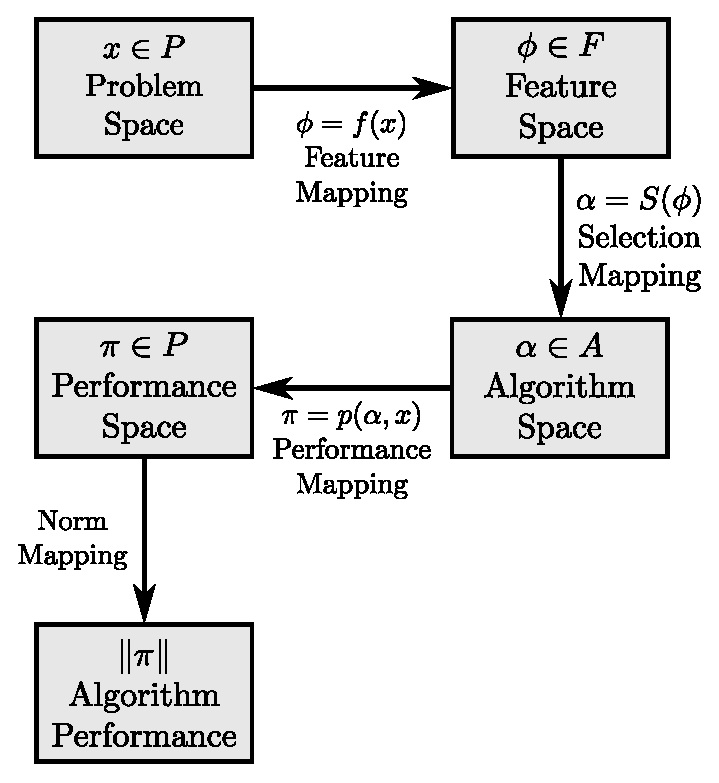
\includegraphics[height=.9\textheight]{algorithm-selection}
    \end{center}
\end{frame}

\begin{frame}
    \frametitle{Autonomous Solvers}
    \begin{center}
        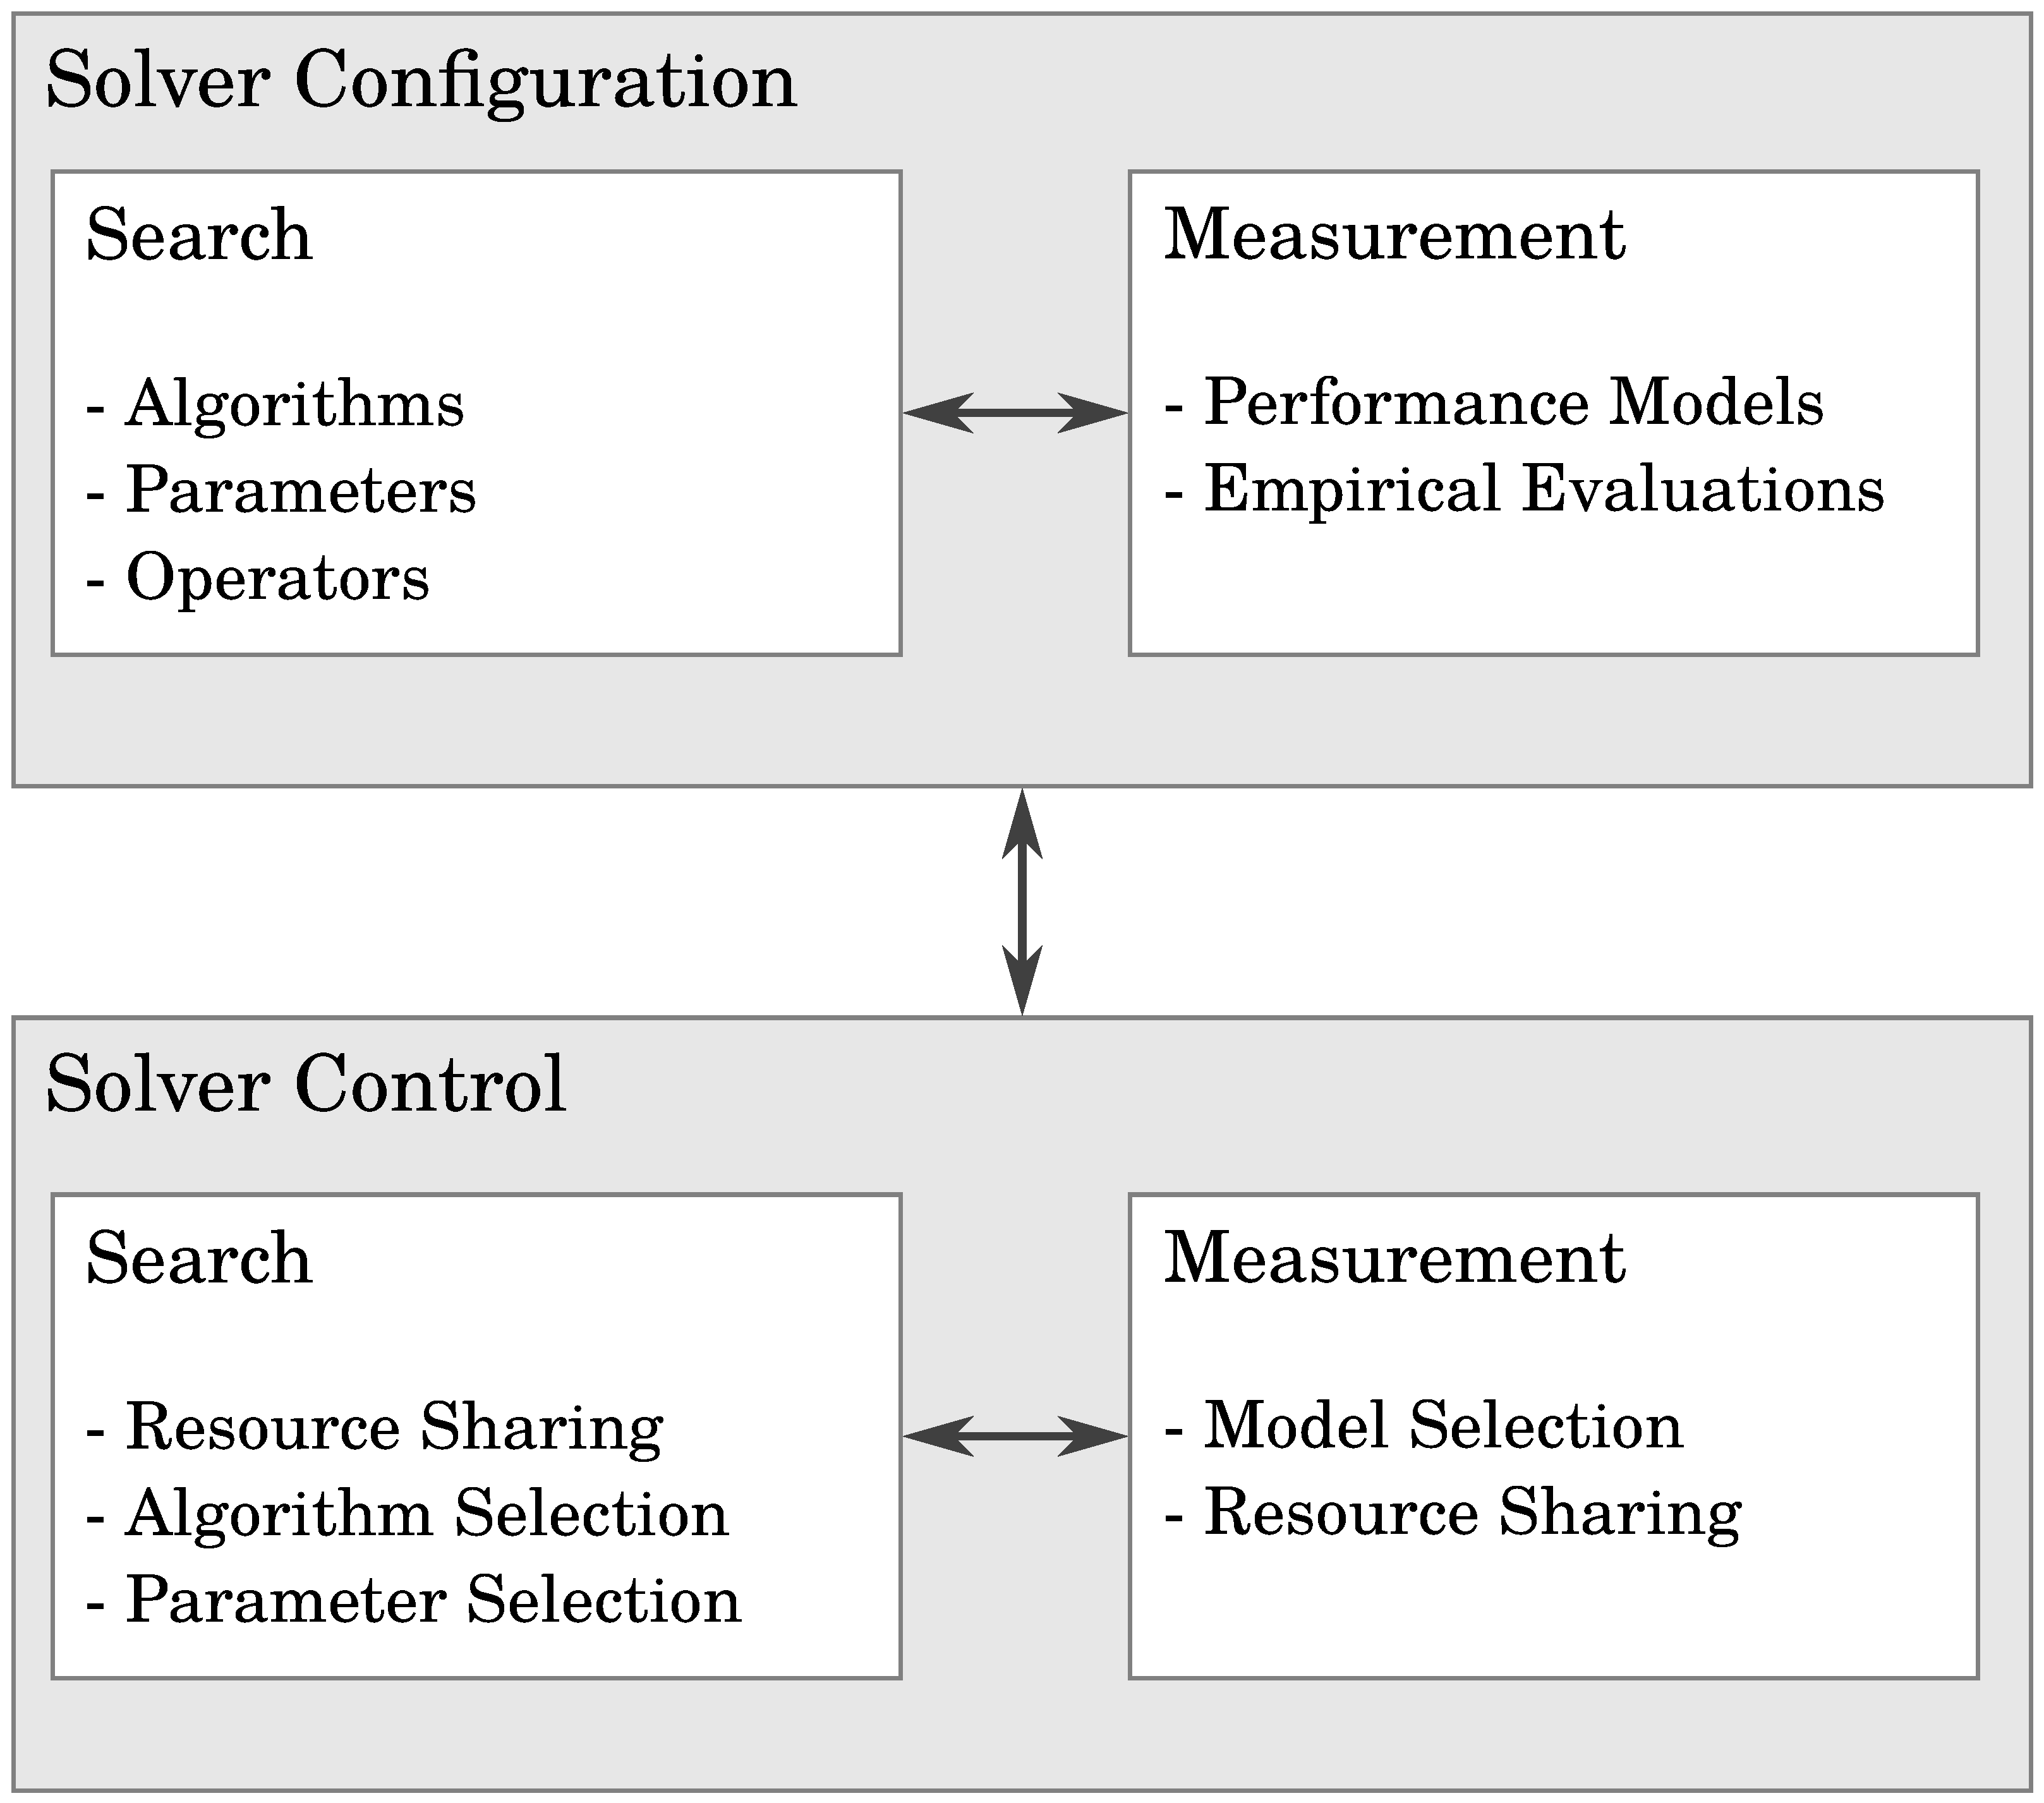
\includegraphics[height=.9\textheight]{general_solver}
    \end{center}
\end{frame}

\begin{frame}
    \frametitle{OpenTuner}
    \begin{center}
        \includegraphics[width=.6\textwidth]{opentuner_arch}
    \end{center}
\end{frame}

\begin{frame}
    \frametitle{OpenTuner: Identified Problems}
        \begin{block}{Identified Problems}
            \begin{center}
                \begin{itemize}
                    \item Python \alert{GIL}
                    \item \alert{Global Result Sharing}
                    \item \alert{Sequential search}
                    \item \alert{Dependent execution flow}
                \end{itemize}
            \end{center}
        \end{block}
\end{frame}

\begin{frame}
    \frametitle{OpenTuner: Identified Problems}
    \begin{center}
        \includegraphics[width=\textwidth]{opentuner_callgraph}
    \end{center}
\end{frame}

\section{Case Studies}
\plain{Case Studies}

\begin{frame}
    \frametitle{Small Measurement Time}
    \begin{center}
        \includegraphics[width=.9\textwidth]{overview_gpus}
    \end{center}
\end{frame}

\begin{frame}
    \frametitle{Key Results}
    \begin{center}
        \includegraphics[width=.9\textwidth]{GPU-tuning-summary}
    \end{center}
\end{frame}

\begin{frame}
    \frametitle{Large Measurement Time}
    \begin{center}
        \includegraphics[width=.8\textwidth]{overview_fpgas_small}
    \end{center}
\end{frame}

\begin{frame}
    \frametitle{Large Measurement Time}
    \begin{center}
        \includegraphics[width=.9\textwidth]{overview_fpgas_big}
    \end{center}
\end{frame}

\begin{frame}
    \frametitle{Key Results}
    \begin{center}
        \includegraphics[width=.9\textwidth]{heatmap_wns_comparison}

        \emph{Relative improvement for \textbf{WNS} in all scenarios}
    \end{center}
\end{frame}

\begin{frame}
    \frametitle{Distributed OpenTuner Extension}
    \begin{center}
        \includegraphics[width=.9\textwidth]{overview_distributed}
    \end{center}
\end{frame}

\begin{frame}
    \frametitle{Dot Product Engine: Hardware \& Software Co-Design}
    \begin{center}
        \includegraphics[width=.9\textwidth]{overview_dpe_hard}
    \end{center}
\end{frame}

\begin{frame}
    \frametitle{Dot Product Engine: Hardware \& Software Co-Design}
    \begin{center}
        \includegraphics[width=.9\textwidth]{overview_dpe_app}
    \end{center}
\end{frame}

\section{NODAL: an Open Distributed Autotuning Library}
\plain{NODAL: an Open Distributed Autotuning Library}

\begin{frame}
    \frametitle{NODAL}
    \begin{columns}[c]
        \column{.45\textwidth}
        \begin{center}
            \includegraphics[width=\columnwidth]{logo}
        \end{center}

        \column{.45\textwidth}
        \begin{block}{NODAL}
            \begin{itemize}
                \item \alert{Open-source}
                \item \alert{Domain-agnostic}
                \item \alert{Parallel \& distributed}
                \item \alert{Ensemble} of search techniques
                \item Written in the \alert{Julia language}
            \end{itemize}
        \end{block}

    \end{columns}
\end{frame}

\begin{frame}
    \frametitle{NODAL}
    \begin{columns}[c]
        \column{.45\textwidth}
        \begin{block}{Problem Representation}
            \begin{itemize}
                \item Parameter \alert{types}
                \item \alert{User-definable cost function}
                \item User-definable \alert{operators}
            \end{itemize}
        \end{block}

        \begin{block}{Robust Search Methods}
            \begin{itemize}
                \item \alert{Combinations} of techniques
                \item \alert{Model-Aided}
                \item \alert{Design of Experiments}
            \end{itemize}
        \end{block}

        \pause

        \column{.45\textwidth}
        \begin{block}{Overcoming Limitations}
            \begin{itemize}
                \item Parallel \alert{search \& measurement}
                \item \alert{Design of Experiments}
            \end{itemize}
        \end{block}

    \end{columns}
\end{frame}

\begin{frame}
    \frametitle{NODAL: The Julia Language}
    \begin{columns}[c]
        \column{.45\textwidth}
        \begin{block}{The Julia Language}
            \begin{itemize}
                \item \alert{High-level abstractions}
                \item \alert{Parallel \& distributed} programming
                \item \alert{High-performance} for a dynamic language
            \end{itemize}
        \end{block}

        \column{.45\textwidth}
        \begin{center}
            \includegraphics[width=.6\columnwidth]{julia}
        \end{center}

    \end{columns}
\end{frame}

\begin{frame}
    \frametitle{NODAL: The Julia Language}
    \begin{center}
        \includegraphics[width=.95\textwidth]{julia_benchmarks}
    \end{center}
\end{frame}

\begin{frame}
    \frametitle{NODAL: Search Techniques}
    \begin{table}
        \centering
        \begin{tabular}{@{}p{.4\textwidth}p{.35\textwidth}@{}}
            \toprule
            \textit{Implemented} & \textit{Planned} \\ \midrule
            Iterative First Improvement & Iterative Best Improvement \\
            Iterative Greedy Construction & Randomized Best Improvement \\
            Iterative Probabilistic Improvement & Randomized Best Improvement \\
            Randomized First Improvement & Iterative Best Construction \\
            Simulated Annealing & Dynamic Local Search \\
            Iterated Local Search & Tabu Search \\
            & Ant Colony Optimization \\
            & Particle Swarm Optimization \\
            & Nelder-Mead \\
            & Genetic Algorithms \\ \bottomrule
        \end{tabular}
    \end{table}
\end{frame}

\begin{frame}
    \frametitle{NODAL: Architecture}
    \begin{center}
        \includegraphics[width=.8\textwidth]{nodal_architecture}
    \end{center}
\end{frame}

\begin{frame}
    \frametitle{NODAL: Execution Flow}
    \begin{center}
        \includegraphics[height=.9\textheight]{nodal_callgraph}
    \end{center}
\end{frame}

\section*{Summary}

\begin{frame}
    \frametitle{Summary}
    \begin{columns}[c]
        \column{.65\textwidth}
        \begin{block}{Domain-Agnostic Autotuning}
            \begin{itemize}
                \item Autotuning as a \alert{search problem}
                \item \alert{Parameters}, \alert{search spaces} \& \alert{cost
                    functions}
                \item Still need to \alert{leverage parallel \& distributed
                    computing}
                \item \alert{Limitations} of current tools
            \end{itemize}
        \end{block}

        \pause

        \column{.3\textwidth}
        \begin{center}
            \includegraphics[width=\columnwidth]{logo}
        \end{center}

    \end{columns}
\end{frame}

\maketitle

\end{document}
